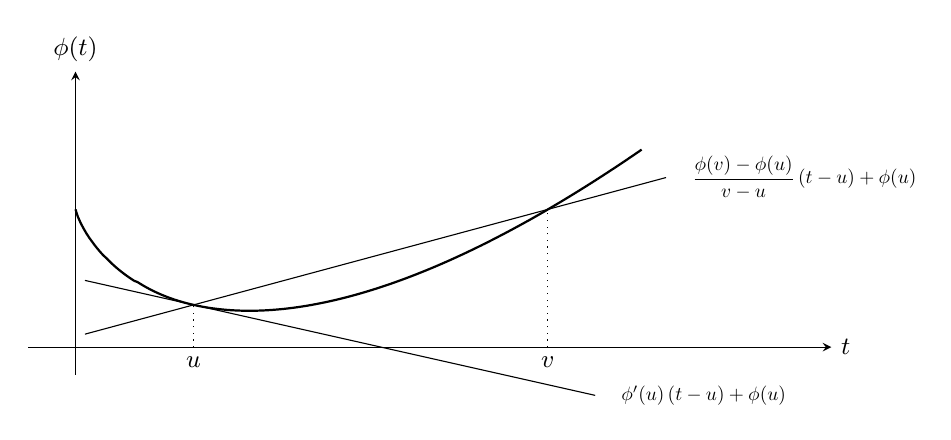
\begin{tikzpicture}[xscale=6,yscale=3.5]
\shorthandoff{>}
%
\pgfmathsetmacro{\u}{.25};
\pgfmathsetmacro{\v}{1};
\pgfmathsetmacro{\dc}{.02};% debut trac� de corde & tangente
\pgfmathsetmacro{\fc}{1.25};% fin trac� de corde
\pgfmathsetmacro{\ft}{1.1};% fin trac� de corde
%
\pgfmathdeclarefunction{sha}{1}{\pgfmathparse{#1*ln(#1)}}
\pgfmathdeclarefunction{shap}{1}{\pgfmathparse{1+ln(#1)}}
%
% Convexidad (t ln t aca)
\draw[>=stealth,->] (-.1,-.5)--(1.6,-.5) node[right]{\small $t$};
\draw[>=stealth,->] (0,-.6)--(0,.5) node[above]{\small $\phi(t)$};
\draw[thick,domain=.005:1.2,samples=200] (0,0)-- plot (\x,{sha(\x)});
\draw[dotted] (\u,-.5) node[below]{\small $u$} -- (\u,{sha(\u)});
\draw[dotted] (\v,-.5) node[below]{\small $v$} -- (\v,{sha(\v)});
%
%\draw[dotted] (\v,-.55) node[below]{\small $v$} -- (\v,{sha(\v)});
%\draw[>=stealth,<->] (\v,{shap(\u)*(\v-\u)+sha(\u)}) -- (\v,{sha(\v)});
%\draw (\v,-.5) node[below right]{\small $v$};
%\draw (\v,{.5*(shap(\u)*(\v-\u)+sha(\u)+sha(\v))}) 
%node[right]{\small $B_\phi(v\|u)$};
%
% Corde entre u et v
\draw (\dc,{(\dc-\u)*(sha(\v)-sha(\u))/(\v-\u)+sha(\u)})
-- (\fc,{(\fc-\u)*(sha(\v)-sha(\u))/(\v-\u)+sha(\u)})
node[right,scale=.7]
{$\displaystyle \quad \frac{\phi(v)-\phi(u)}{v-u} \, (t-u) + \phi(u)$};;
%
% tangente
\draw (\dc,{shap(\u)*(\dc-\u)+sha(\u)})--(\ft,{shap(\u)*(\ft-\u)+sha(\u)})
node[right,scale=.7]{$\quad \phi'(u) \, (t-u) + \phi(u)$};
%
\end{tikzpicture}